\newpage
\subsection{Results}

Using the proposed model, the first step is to understand the main component of the commuting dynamic. The result of our approach will emerge from this main component as we can see in the next pictures. This main component model the first logic result and shows the time segments that people have more activite, in call numbers terms.

\begin{figure}[ht]
\centering
\subfigure[Total number of calls grouped by Week days]{
	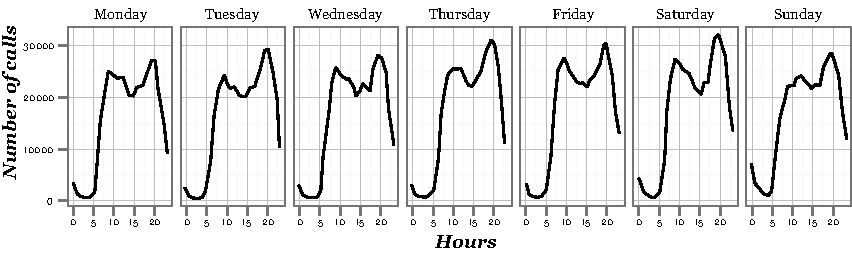
\includegraphics[scale =0.4] {results/images/calls_number.pdf}
	\label{fig:subfig11}
}
\label{fig:fig1}
\end{figure}


enlazar con que apartir de esta componente temporal, demostramos los picos de lomngitus y un mayor valle central.